\documentclass{ximera}

\input{../preamble.tex}



\title{5.2 - Trigonometric identities, graphs, and limits}

\begin{document}
\begin{abstract}
  We introduce the identities and graphs of trigonometric functions.
\end{abstract}
\maketitle

\section{The power of the Pythagorean Theorem}

The Pythagorean Theorem is probably the most famous theorem in all of
mathematics.

\begin{theorem}[Pythagorean Theorem]\index{Pythagorean Theorem}
Given a right triangle:
\begin{image}[2in]
  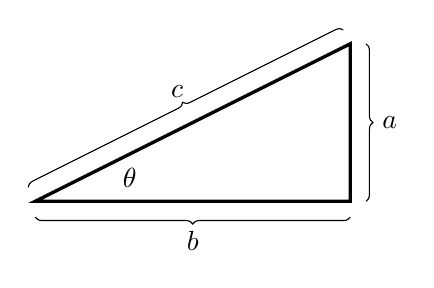
\begin{tikzpicture}
    \coordinate (C) at (0,2);
    \coordinate (D) at (4,2);
    \coordinate (E) at (4,4);
    \tkzMarkRightAngle(C,D,E)
    \tkzMarkAngle(D,C,E)
    \draw[decoration={brace,mirror,raise=.2cm},decorate,thin] (0,2)--(4,2);
    \draw[decoration={brace,mirror,raise=.2cm},decorate,thin] (4,2)--(4,4);
    \draw[decoration={brace,raise=.2cm},decorate,thin] (0,2)--(4,4);
    \draw[very thick] (D)--(E)--(C)--cycle;
    \node at (2,2-.5) {$b$};
    \node[] at (4+.5,3) {$a$};
    \node at (2-.2,3+.4) {$c$};
    \node at (1.2,2.3) {$\theta$};
  \end{tikzpicture}
\end{image}
We have that:
\[
a^2 + b^2 = c^2
\]
\end{theorem}


The Pythagorean Theorem gives several key trigonometric identities.

\begin{theorem}[Pythagorean Identities]\index{Pythagorean identities}
  The following hold:
  \[
  \cos^2(\theta)+\sin^2(\theta) = 1 \qquad 1 + \tan^2(\theta) = \sec^2(\theta) \qquad \cot^2(\theta) + 1 = \csc^2(\theta)
  \]
  \begin{explanation}
    From the unit circle we can see
    \begin{image}
	\begin{tikzpicture}
	\begin{axis}[
            xmin=-1.1,xmax=1.1,ymin=-1.1,ymax=1.1,
            axis lines=center,
            width=4in,
            ticks=none,
            clip=false,
            unit vector ratio*=1 1 1,
            %xlabel=$x$, ylabel=$y$,
            every axis y label/.style={at=(current axis.above origin),anchor=south},
            every axis x label/.style={at=(current axis.right of origin),anchor=west},
          ]        
          \addplot [dashed, smooth, domain=(0:360)] ({cos(x)},{sin(x)}); %% unit circle

          \addplot [textColor] plot coordinates {(0,0) (.766,.643)}; %% 40 degrees

          \addplot [ultra thick,penColor] plot coordinates {(.766,0) (.766,.643)}; %% 40 degrees
          \addplot [ultra thick,penColor2] plot coordinates {(0,0) (.766,0)}; %% 40 degrees
          
          %\addplot [ultra thick,penColor3] plot coordinates {(1,0) (1,.839)}; %% 40 degrees          

          \addplot [textColor,smooth, domain=(0:40)] ({.15*cos(x)},{.15*sin(x)});
          %\addplot [very thick,penColor] plot coordinates {(0,0) (.766,.643)}; %% sector
          %\addplot [very thick,penColor] plot coordinates {(0,0) (1,0)}; %% sector
          %\addplot [very thick, penColor, smooth, domain=(0:40)] ({cos(x)},{sin(x)}); %% sector
          \node at (axis cs:.15,.07) [anchor=west] {$t$};
          \node[penColor, rotate=-90] at (axis cs:.84,.322) {$\sin(t)$};
          \node[penColor2] at (axis cs:.383,0) [anchor=north] {$\cos(t)$};
          %\node[penColor3, rotate=-90] at (axis cs:1.06,.322) {$\tan(\theta)$};
        	\end{axis}
	\end{tikzpicture}
    \end{image}
    via the Pythagorean Theorem that
    \[
    \cos^2(t) + \sin^2(t) = 1.
    \]
    If we divide this expression by $\answer[given]{\cos^2(t)}$ we obtain
    \[
    1 + \tan^2(t) = \sec^2(t)
    \]
    and if we divide $\cos^2(t) + \sin^2(t) = 1$ by $\answer[given]{\sin^2(t)}$ we obtain
    \[
    \cot^2(t) + 1 = \csc^2(t).
    \]
  \end{explanation}
\end{theorem}

There several other trigonometric identities that appear on occasion.
\begin{theorem}[Angle Addition Formulas]\index{Angle addition formulas}
	\begin{align*}
		\sin(s + t) &= \sin(s)\cos(t)  + \cos(s)\sin(t) \\
		\cos(s+t) &= \cos(s)\cos(t) - \sin(s)\sin(t)
	\end{align*}
\end{theorem}

If we plug $s = t = \theta$ into the angle addition formulas, we find the double-angle identities.
\begin{theorem}[Double-Angle Identities]\index{Double-angle identities}
	\begin{align*}
		\sin(2 \theta) &= 2\sin(\theta)\cos(\theta)\\
		\cos(2\theta) &= \cos^2(\theta) - \sin^2(\theta)\\
			&= 2 \cos^2(\theta)-1\\
			&= 1 - 2 \sin^2(\theta)
	\end{align*}
\end{theorem}

Solving the bottom two formulas for $\cos^2(\theta)$ and $\sin^2(\theta)$ gives the half-angle identities.
\begin{theorem}[Half-Angle Identities]\index{Half-angle identities}
	\begin{align*}
		\sin^2(\theta) &= \frac{1-\cos(2\theta)}{2}\\
		\cos^2(\theta) &= \frac{1+\cos(2\theta)}{2}	
	\end{align*}
\end{theorem}

\begin{theorem}[Cofunction Identities]
	\begin{align*}
		\cos(\theta) &= \sin(\pi/2-\theta)\\
		\sin(\theta) &= \cos(\pi/2-\theta)
	\end{align*}
\end{theorem}

\section{Trigonometric equations}
Frequently we are in the situation of having to determine precisely which angles satisfy a particular equation.  The most basic example is probably like this one.
\begin{example}
	Solve the equation: \[ \sin(\theta) = -\frac{1}{2}. \]
	\begin{explanation}
		We'll start by finding the reference angle, $\theta_R$, the acute angle between the terminal side of $\theta$ and the $x$-axis.  
		The reference angle satisfies $\sin(\theta_R) = \frac{1}{2}$.  
		\begin{image}[2in]
		   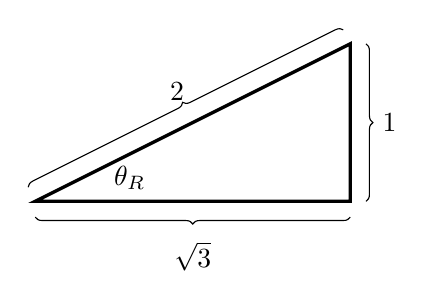
\begin{tikzpicture}
    			\coordinate (C) at (0,2);
    			\coordinate (D) at (4,2);
   			 \coordinate (E) at (4,4);
   			 \tkzMarkRightAngle(C,D,E)
    			\tkzMarkAngle(D,C,E)
    			\draw[decoration={brace,mirror,raise=.2cm},decorate,thin] (0,2)--(4,2);
   			 \draw[decoration={brace,mirror,raise=.2cm},decorate,thin] (4,2)--(4,4);
  			  \draw[decoration={brace,raise=.2cm},decorate,thin] (0,2)--(4,4);
  			  \draw[very thick] (D)--(E)--(C)--cycle;
    			\node at (2,2-.7) {$\answer{\sqrt{3}}$};
    			\node[] at (4+.5,3) {$1$};
    			\node at (2-.2,3+.4) {$2$};
    			\node at (1.2,2.3) {$\theta_R$};
  		  \end{tikzpicture}
		\end{image}
		From the picture (or from our knowledge of the unit circle) we determine that our reference angle is $\theta_R = \frac{\pi}{6}$.  In one rotation $[0, 2\pi]$, there are two angles that have reference angle $\frac{\pi}{6}$ and have negative
		sine value (since we are solving $\sin(\theta) = -\frac{1}{2}$).  One is in quadrant 3, and one in quadrant 4.  That means the solutions in the interval $[0, 2\pi]$ are $\frac{5\pi}{6}$ and $\frac{11\pi}{6}$.
		
		Notice that any angle whose terminal side falls in either of these positions also solution to $\sin(\theta) = -\frac{1}{2}$. To include these angles, we add all integer-multiples of $2\pi$ to our two previous angles.
		 The solutions are then \[ \theta = \frac{5\pi}{6} + 2\pi k , \,\, \frac{11\pi}{6}+2\pi k , \,\, k \textrm{ any integer}. \]
	\end{explanation}
\end{example}

\begin{problem}
	Solve the equation: \[ \tan(\theta) = -\sqrt{3}. \]
	\begin{multipleChoice}
		\choice{$\theta = \frac{\pi}{3}+\pi k$}
		\choice{$\theta = \frac{\pi}{6}+ \pi k$}
		\choice[correct]{$\theta = \frac{2\pi}{3}+ \pi k$}
		\choice{$\theta = \frac{5\pi}{6}+\pi k$}
		\choice{None of the above}
	\end{multipleChoice}
\end{problem}

%Let's try one a bit more complicated.
%\begin{example}
%	Solve the equation: \[ \cos(\theta) \left( \cos(\theta) + 1\right) = \sin^2(\theta). \]
%	\begin{explanation}
%		We'll start by simplifying a bit.
%		\begin{align*}
%			\cos(\theta) \left( \cos(\theta) + 1\right) &= \sin^2(\theta) \\
%			\cos^2(\theta) + \cos(\theta) &= \sin^2(\theta) \\
%			\cos^2(\theta) - \sin^2(\theta) + \cos(\theta) &= 0\\
%			\cos^2(\theta) - \left(1-\cos^2\theta\right) + \cos(\theta) &= 0\\
%			2\cos^2(\theta) + \cos(\theta) - 1 &= 0.
%		\end{align*}
%		Notice that this equation is quadratic in $\cos(\theta)$.  We can factor it like we try to do to solve any other quadratic equation:
%		\[ \left( \cos(\theta) + 1 \right) \left( 2 \cos(\theta) - 1\right) = 0.\]
%		On the interval $[0, 2\pi]$, $\cos(\theta) = -1$ has only one solution, $\theta = \answer[given]{\pi}$.  
%		For $\cos(\theta) = \frac{1}{2}$, we see that the reference angle $\theta_R = \answer[given]{\frac{\pi}{3}}$.  Since cosine is positive in quadrants 1 and 4,
%		we find solutions $\theta = \frac{\pi}{3}$ and $\frac{5\pi}{3}$.
%		
%		All solutions are:
%		\[ \theta = \pi + 2 \pi k, \,\, \frac{\pi}{3}+ 2 \pi k ,\,\, \frac{5\pi}{3} + 2\pi k, \,\, k \textrm{ any integer.} \]
%	\end{explanation}
%\end{example}


\section{Graphs}
Below are the graphs of the six trigonometric functions. Remember that while the unit circle is an image of $(x,y)=(\cos(\theta),\sin(\theta))$ points, the graph of $y=\cos(\theta)$, for example, takes angle $\theta$ as the input and plots its cosine value as the output, or height. As we increase the angle and swing around the unit circle, all six trig functions start to repeat the same numbers in the same order. Thus, all six of these graphs are \dfn{periodic}.

\begin{image}
\begin{tikzpicture}
	\begin{axis}[
            xmin=-6.75,xmax=6.75,ymin=-1.5,ymax=1.5,
            axis lines=center,
            xtick={-6.28, -4.71, -3.14, -1.57, 0, 1.57, 3.142, 4.71, 6.28},
            xticklabels={$-2\pi$,$-3\pi/2$,$-\pi$, $-\pi/2$, $0$, $\pi/2$, $\pi$, $3\pi/2$, $2\pi$},
            ytick={-1,1},
            %ticks=none,
            width=6in,
            height=3in,
            unit vector ratio*=1 1 1,
            xlabel=$\theta$, ylabel=$y$,
            every axis y label/.style={at=(current axis.above origin),anchor=south},
            every axis x label/.style={at=(current axis.right of origin),anchor=west},
          ]        
          \addplot [very thick, penColor, samples=300,smooth, domain=(-6.75:6.75)] {sin(deg(x))};
          \node at (axis cs:-1.57,.75) [penColor2] {$y=\sin(\theta)$};
        \end{axis}
\end{tikzpicture}
\end{image}

\begin{image}
\begin{tikzpicture}
	\begin{axis}[
            xmin=-6.75,xmax=6.75,ymin=-1.5,ymax=1.5,
            axis lines=center,
            xtick={-6.28, -4.71, -3.14, -1.57, 0, 1.57, 3.142, 4.71, 6.28},
            xticklabels={$-2\pi$,$-3\pi/2$,$-\pi$, $-\pi/2$, $0$, $\pi/2$, $\pi$, $3\pi/2$, $2\pi$},
            ytick={-1,1},
            %ticks=none,
            width=6in,
            height=3in,
            unit vector ratio*=1 1 1,
            xlabel=$\theta$, ylabel=$y$,
            every axis y label/.style={at=(current axis.above origin),anchor=south},
            every axis x label/.style={at=(current axis.right of origin),anchor=west},
          ]        
          \addplot [very thick, penColor, samples=300,smooth, domain=(-6.75:6.75)] {cos(deg(x))};
          \node at (axis cs:-1.8,.75) [penColor2] {$y=\cos(\theta)$};
        \end{axis}
\end{tikzpicture}
\end{image}

Notice that both $y=\sin(\theta)$ and $y=\cos(\theta)$ have domain $(-\infty,\infty)$ and range $[-1,1]$.

\begin{image}
\begin{tikzpicture}
	\begin{axis}[
            xmin=-6.75,xmax=6.75,ymin=-5.5,ymax=5.5,
            axis lines=center,
            xtick={-6.28, -4.71, -3.14, -1.57, 0, 1.57, 3.142, 4.71, 6.28},
            xticklabels={$-2\pi$,$-3\pi/2$,$-\pi$, $-\pi/2$, $0$, $\pi/2$, $\pi$, $3\pi/2$, $2\pi$},
            ytick={-1,1},
            %ticks=none,
            width=6in,
            height=3in,
            unit vector ratio*=1 1 1,
            xlabel=$\theta$, ylabel=$y$,
            every axis y label/.style={at=(current axis.above origin),anchor=south},
            every axis x label/.style={at=(current axis.right of origin),anchor=west},
          ]        
          \addplot [very thick, penColor, samples=100,smooth, domain=(-1.56:1.56)] {tan(deg(x))};
          \addplot [very thick, penColor, samples=100,smooth, domain=(1.58:4.7)] {tan(deg(x))};
          \addplot [very thick, penColor, samples=100,smooth, domain=(4.9:6.28)] {tan(deg(x))};
          \addplot [very thick, penColor, samples=100,smooth, domain=(-4.7:-1.58)] {tan(deg(x))};
          \addplot [very thick, penColor, samples=100,smooth, domain=(-6.28:-4.9)] {tan(deg(x))};          
          \node at (axis cs:-0.5,2) [penColor2] {$y=\tan(\theta)$};
          
          \addplot [textColor, dashed] plot coordinates {(-4.7124,-5.5) (-4.7124,5.5)};
          \addplot [textColor, dashed] plot coordinates {(-1.57,-5.5) (-1.57,5.5)};          
          \addplot [textColor, dashed] plot coordinates {(1.57,-5.5) (1.57,5.5)}; 
          \addplot [textColor, dashed] plot coordinates {(4.7124,-5.5) (4.7124,5.5)};          
        \end{axis}
\end{tikzpicture}
\end{image}
Notice that $y=\tan(\theta)=\frac{\sin(\theta)}{\cos(\theta)}$ is undefined whenever $\cos(\theta)=0$. Because it is division by zero, we see vertical asymptotes in the graph. Thus the domain of $y=\tan(\theta)$ is all numbers except $\theta=\pi/2+\pi k$ for any integer $k$. Its range is $(-\infty,\infty)$. The remaining three graphs all have vertical asymptotes at angles that correspond to division by zero.

\begin{image}
\begin{tikzpicture}
	\begin{axis}[
            xmin=-6.75,xmax=6.75,ymin=-5.5,ymax=5.5,
            axis lines=center,
            xtick={-6.28, -4.71, -3.14, -1.57, 0, 1.57, 3.142, 4.71, 6.28},
            xticklabels={$-2\pi$,$-3\pi/2$,$-\pi$, $-\pi/2$, $0$, $\pi/2$, $\pi$, $3\pi/2$, $2\pi$},
            ytick={-1,1},
            %ticks=none,
            width=6in,
            height=3in,
            unit vector ratio*=1 1 1,
            xlabel=$\theta$, ylabel=$y$,
            every axis y label/.style={at=(current axis.above origin),anchor=south},
            every axis x label/.style={at=(current axis.right of origin),anchor=west},
          ]        
          \addplot [very thick, penColor, samples=100,smooth, domain=(3.15:6.27)] {cot(deg(x))};
          \addplot [very thick, penColor, samples=100,smooth, domain=(0.01:3.13)] {cot(deg(x))};
          \addplot [very thick, penColor, samples=100,smooth, domain=(-3.13:-0.01)] {cot(deg(x))};
          \addplot [very thick, penColor, samples=100,smooth, domain=(-6.27:-3.15)] {cot(deg(x))};          
          \node at (axis cs:-0.7,2) [penColor2] {$y=\cot(\theta)$};
          
          \addplot [textColor, dashed] plot coordinates {(-6.2832,-5.5) (-6.2832,5.5)};
          \addplot [textColor, dashed] plot coordinates {(-3.1416,-5.5) (-3.14156,5.5)};          
          \addplot [textColor, dashed] plot coordinates {(3.1416,-5.5) (3.1416,5.5)}; 
          \addplot [textColor, dashed] plot coordinates {(6.2832,-5.5) (6.2832,5.5)};      
          
          \end{axis}
\end{tikzpicture}
\end{image}


\begin{image}
\begin{tikzpicture}
	\begin{axis}[
            xmin=-6.75,xmax=6.75,ymin=-5.5,ymax=5.5,
            axis lines=center,
            xtick={-6.28, -4.71, -3.14, -1.57, 0, 1.57, 3.142, 4.71, 6.28},
            xticklabels={$-2\pi$,$-3\pi/2$,$-\pi$, $-\pi/2$, $0$, $\pi/2$, $\pi$, $3\pi/2$, $2\pi$},
            ytick={-1,1},
            %ticks=none,
            width=6in,
            height=3in,
            unit vector ratio*=1 1 1,
            xlabel=$\theta$, ylabel=$y$,
            every axis y label/.style={at=(current axis.above origin),anchor=south},
            every axis x label/.style={at=(current axis.right of origin),anchor=west},
          ]        
          \addplot [very thick, penColor, samples=100,smooth, domain=(-1.56:1.56)] {sec(deg(x))};
          \addplot [very thick, penColor, samples=100,smooth, domain=(1.58:4.7)] {sec(deg(x))};
          \addplot [very thick, penColor, samples=100,smooth, domain=(4.9:6.28)] {sec(deg(x))};
          \addplot [very thick, penColor, samples=100,smooth, domain=(-4.7:-1.58)] {sec(deg(x))};
          \addplot [very thick, penColor, samples=100,smooth, domain=(-6.28:-4.9)] {sec(deg(x))};          
          \node at (axis cs:-2.0,0.5) [penColor2] {$y=\sec(\theta)$};
           \addplot [textColor, dashed] plot coordinates {(-4.7124,-5.5) (-4.7124,5.5)};
          \addplot [textColor, dashed] plot coordinates {(-1.57,-5.5) (-1.57,5.5)};          
          \addplot [textColor, dashed] plot coordinates {(1.57,-5.5) (1.57,5.5)}; 
          \addplot [textColor, dashed] plot coordinates {(4.7124,-5.5) (4.7124,5.5)};      
        \end{axis}
\end{tikzpicture}
\end{image}

\begin{image}
\begin{tikzpicture}
	\begin{axis}[
            xmin=-6.75,xmax=6.75,ymin=-5.5,ymax=5.5,
            axis lines=center,
            xtick={-6.28, -4.71, -3.14, -1.57, 0, 1.57, 3.142, 4.71, 6.28},
            xticklabels={$-2\pi$,$-3\pi/2$,$-\pi$, $-\pi/2$, $0$, $\pi/2$, $\pi$, $3\pi/2$, $2\pi$},
            ytick={-1,1},
            %ticks=none,
            width=6in,
            height=3in,
            unit vector ratio*=1 1 1,
            xlabel=$\theta$, ylabel=$y$,
            every axis y label/.style={at=(current axis.above origin),anchor=south},
            every axis x label/.style={at=(current axis.right of origin),anchor=west},
          ]        
          \addplot [very thick, penColor, samples=100,smooth, domain=(3.15:6.27)] {1/sin(deg(x))};
          \addplot [very thick, penColor, samples=100,smooth, domain=(0.01:3.13)] {1/sin(deg(x))};
          \addplot [very thick, penColor, samples=100,smooth, domain=(-3.13:-0.01)] {1/sin(deg(x))};
          \addplot [very thick, penColor, samples=100,smooth, domain=(-6.27:-3.15)] {1/sin(deg(x))};          
          \node at (axis cs:-1.2,2) [penColor2] {$y=\csc(\theta)$};
          \addplot [textColor, dashed] plot coordinates {(-6.2832,-5.5) (-6.2832,5.5)};
          \addplot [textColor, dashed] plot coordinates {(-3.1416,-5.5) (-3.14156,5.5)};          
          \addplot [textColor, dashed] plot coordinates {(3.1416,-5.5) (3.1416,5.5)}; 
          \addplot [textColor, dashed] plot coordinates {(6.2832,-5.5) (6.2832,5.5)};               
        \end{axis}
\end{tikzpicture}
\end{image}

Notice that since $y=\sec(\theta)=\frac{1}{\cos(\theta)}$, like $y=\tan(\theta)$, has division by $\cos(\theta)$, its domain is all numbers except $\pi/2+\pi k$ for any integer $k$. S ince $y=\csc(\theta)=\frac{1}{\sin(\theta)}$ has division by $\sin(\theta)$, its domain is all numbers except $0+\pi k$ for any integer $k$. Both $y=\sec(\theta)$ and $y=\csc(\theta)$ have range $(-\infty,-1]\cup[1,\infty)$. Finally, $y=\cot(\theta)$ has domain all numbers except $0+\pi k$ for any integer $k$ and range $(-\infty,\infty)$.

\section{Limits involving trigonometric functions}
It can be proven that each trigonometric function is continuous on its domain. We can use this information, combined with the graphs above, to compute some interesting limits.

\begin{example}
	Compute the limit: \[ \lim_{\theta \to 2\pi/3} \theta \tan(\theta). \]
	\begin{explanation}
		Assuming each limit exists (which they do), the multiplicative limit law allows us to split this into \[ \left(\lim_{\theta\to 2\pi/3} \theta \right) \left(\lim_{\theta\to 2\pi/3} \tan(\theta) \right). \]
		The function $f(\theta) = \theta$ is continuous everywhere, so $\lim_{\theta\to 2\pi/3} \theta = \answer[given]{\frac{2\pi}{3}}$.  Since $\frac{2 \pi}{3}$ is in the domain
		of $\tan(\theta)$, we have $\lim_{\theta\to 2\pi/3} \tan(\theta) = \tan \left( \answer[given]{\frac{2 \pi}{3}} \right) = - \sqrt{3}$.  Putting these together we find
		\[ \lim_{\theta\to 2\pi/3} \theta \tan(\theta) = - \frac{2 \pi \sqrt{3}}{3}. \]
	\end{explanation}
\end{example}


\begin{example}
	Compute the limit: \[ \lim_{\theta \to \pi^-} \cot(\theta). \]
	\begin{explanation}
		Recall that $\cot(\theta) = \frac{\cos(\theta)}{\sin(\theta)}$, so that \[ \lim_{\theta \to \pi^-} \cot(\theta) = \lim_{\theta \to \pi^-} \frac{\cos(\theta)}{\sin(\theta)}.\]
		Since sine and cosine are continuous, $\lim_{\theta \to \pi^-} \cos(\theta) = \cos\left( \answer[given]{\pi} \right)= \answer[given]{-1}$ and 
		$\lim_{\theta \to \pi^-} \sin(\theta) = \sin\left( \answer[given]{\pi} \right)  = \answer[given]{0}$.
		That is, $\lim_{\theta \to \pi^-} \cot(\theta)$ is of the form $\numOverZero$.
		
		The numerator is negative for $\theta$ near $\pi$.  From the graph of $\sin(\theta)$, we know that the denominator is negative and approaching $0$ as $\theta \to \pi^{-}$.
		That means \[ \lim_{\theta \to \pi^-} \cot(\theta) = -\infty. \]
	\end{explanation}
\end{example}

Because for all $x$, $-1\leq\cos(x)\leq 1$ and $-1\leq\sin(x)\leq 1$, limits involving trig functions are excellent applications of the Squeeze Theorem.

\begin{example}
	Compute the limit: 
	\[ \lim_{x \to \infty } \frac{ \sin(x)}{x^2} \]
	\begin{explanation}
	Since for all $x$, we know that $-1\leq\sin(x)\leq 1$, we can write
	\[ \frac{-1}{x^2}\leq\frac{\sin(x)}{x^2}\leq\frac{1}{x^2}\]
	for $x>0$. Since 
	\[\lim_{x \to \infty } \frac{-1}{x^2}=\lim_{x \to \infty } \frac{1}{x^2}=0,\]
	by the Squeeze Theorem we can conclude that  \(\lim_{x \to \infty } \frac{ \sin(x)}{x^2}=0\) as well.
	\\This information tells us that $y=\frac{\sin(x)}{x^2}$ has a horizontal asymptote at $y=0$. Interestingly, due to the $\sin(x)$ component the graph oscillates about this asymptote, as shown below.
	
\begin{image}	\begin{tikzpicture} [scale=.5]
    \begin{axis}[samples=50,xmin=0,xmax=27, ymin=-.1, ymax=.1, axis x line= middle, axis y line = middle,xtick={},ytick={}]
	\addplot[black,domain=2:25,<->] {sin(deg(x))/(x^2)};
	\end{axis}
\end{tikzpicture}\end{image}
	
	\end{explanation}
\end{example}

\begin{example}
Compute:
\[
\lim_{\theta\to 0} \frac{\sin(\theta)}{\theta}
\]
\begin{explanation}
To compute this limit, use the Squeeze Theorem in a more creative way. First note that we
only need to examine $\theta\in \left(\frac{-\pi}{2}, \frac{\pi}{2}\right)$
and for the present time, we'll assume that $\theta$ is positive. Consider
the diagrams below:

\begin{tabular}{ccc}
\begin{tikzpicture}
	\begin{axis}[
            xmin=-.1,xmax=1.1,ymin=-.1,ymax=1.1,
            axis lines=center,
            ticks=none,
            clip=false,
            unit vector ratio*=1 1 1,
            xlabel=$x$, ylabel=$y$,
            every axis y label/.style={at=(current axis.above origin),anchor=south},
            every axis x label/.style={at=(current axis.right of origin),anchor=west},
          ]        
          \addplot [very thick, penColor2, smooth, domain=(-.1:.2+pi/2)] ({cos(deg(x))},{sin(deg(x))});
          \addplot [textColor] plot coordinates {(0,0) (1,.839)}; %% 40 degrees
          \addplot [very thick, penColor] plot coordinates {(.766,0) (.766,.643)}; %% 40 degrees
          \addplot [textColor] plot coordinates {(1,0) (1,.839)}; %% 40 degrees
          \addplot [very thick,penColor,fill=fill1] plot coordinates {(0,0) (.766,.643)}\closedcycle; %% triangle
          \addplot [textColor,smooth, domain=(0:40)] ({.15*cos(x)},{.15*sin(x)});
          \node at (axis cs:.15,.07) [anchor=west] {$\theta$};
          \node at (axis cs:.766,.322) [anchor=east] {$\sin(\theta)$};
          \node at (axis cs:.383,0) [anchor=north] {$\cos(\theta)$};
          \node at (axis cs:.5,-.1) [anchor=north] {Triangle $A$};
        \end{axis}
\end{tikzpicture} & 
\begin{tikzpicture}
  \begin{axis}[
      clip=false,
      xmin=-.1,xmax=1.1,ymin=-.1,ymax=1.1,
      axis lines=center,
      ticks=none,
      unit vector ratio*=1 1 1,
      xlabel=$x$, ylabel=$y$,
      every axis y label/.style={at=(current axis.above origin),anchor=south},
      every axis x label/.style={at=(current axis.right of origin),anchor=west},
    ]        
    \addplot [draw=none,fill=fill1] plot coordinates {(0,0) (.766,.643)}\closedcycle; %% sector
    \addplot [draw=none, fill=fill1, samples=100, domain=(0:40)] ({cos(x)},{sin(x)})\closedcycle; %% sector 
    \addplot [very thick, penColor2, smooth, domain=(-.1:.2+pi/2)] ({cos(deg(x))},{sin(deg(x))});
    \addplot [textColor] plot coordinates {(0,0) (1,.839)}; %% 40 degrees
    \addplot [textColor] plot coordinates {(.766,0) (.766,.643)}; %% 40 degrees
    \addplot [textColor] plot coordinates {(1,0) (1,.839)}; %% 40 degrees          
    \addplot [textColor,smooth, domain=(0:40)] ({.15*cos(x)},{.15*sin(x)});
    \addplot [very thick,penColor] plot coordinates {(0,0) (.766,.643)}; %% sector
    \addplot [very thick,penColor] plot coordinates {(0,0) (1,0)}; %% sector
    \addplot [very thick, penColor, smooth, domain=(0:40)] ({cos(x)},{sin(x)}); %% sector
    \node at (axis cs:.15,.07) [anchor=west] {$\theta$};
    \node at (axis cs:.5,0) [anchor=north] {$1$};
    \node at (axis cs:.5,-.1) [anchor=north] {Sector};
  \end{axis}
\end{tikzpicture}  & 
\begin{tikzpicture}
  \begin{axis}[
      clip=false,
      xmin=-.1,xmax=1.1,ymin=-.1,ymax=1.1,
      axis lines=center,
      ticks=none,
      unit vector ratio*=1 1 1,
      xlabel=$x$, ylabel=$y$,
      every axis y label/.style={at=(current axis.above origin),anchor=south},
      every axis x label/.style={at=(current axis.right of origin),anchor=west},
    ]        
    \addplot [very thick,penColor,fill=fill1] plot coordinates {(0,0) (1,.839)}\closedcycle; %% triangle          
    \addplot [very thick, penColor2, smooth, domain=(-.1:1.671)] ({cos(deg(x))},{sin(deg(x))});
    \addplot [very thick, penColor] plot coordinates {(0,0) (1,.839)}; %% 40 degrees
    \addplot [textColor] plot coordinates {(.766,0) (.766,.643)}; %% 40 degrees
    \addplot [very thick, penColor] plot coordinates {(1,0) (1,.839)}; %% 40 degrees          
    \addplot [textColor,smooth, domain=(0:40)] ({.15*cos(x)},{.15*sin(x)});
    \node at (axis cs:.15,.07) [anchor=west] {$\theta$};
    \node at (axis cs:.5,0) [anchor=north] {$1$};
    \node at (axis cs:1,.42) [anchor=west] {$\tan(\theta)$};
    \node at (axis cs:.5,-.1) [anchor=north] {Triangle $B$};
  \end{axis}
\end{tikzpicture}
\end{tabular}



From our diagrams above we see that
\[
\text{Area of Triangle $A$} \le \text{Area of Sector} \le \text{Area of Triangle $B$}
\]
and computing these areas we find
\[
\frac{\cos(\theta)\sin(\theta)}{2} \le \frac{\theta}{2} \le \frac{\tan(\theta)}{2}.
\]
Multiplying through by $2$, and recalling that $\tan(\theta) =
\frac{\sin(\theta)}{\cos(\theta)}$ we obtain
\[
\cos(\theta)\sin(\theta) \le \theta \le \frac{\sin(\theta)}{\cos(\theta)}.
\]
Dividing through by $\sin(\theta)$ and taking the reciprocals
(reversing the inequalities), we find
\[
\cos(\theta) \le \frac{\sin(\theta)}{\theta} \le \frac{1}{\cos(\theta)}.
\]
Note, $\cos(-\theta) = \cos(\theta)$ and $\frac{\sin(-\theta)}{-\theta} =
\frac{\sin(\theta)}{\theta}$, so these inequalities hold for all $\theta\in
\left(\frac{-\pi}{2}, \frac{\pi}{2}\right)$.  Additionally, we know
\[
\lim_{\theta \to 0}\cos(\theta) = \answer[given]{1} = \lim_{\theta\to 0}\frac{1}{\cos(\theta)},
\]
and so we conclude by the Squeeze Theorem, $\lim_{\theta \to
  0}\frac{\sin(\theta)}{\theta} = \answer[given]{1}$.
\end{explanation}
\end{example}

%When solving a problem with the Squeeze Theorem, one must write a sort of mathematical poem. You have to tell your friendly reader exactly which functions you are using to ``squeeze-out'' your limit.

%\begin{example}
%  Compute:
%  \[
%  \lim_{x\to 0} \left(\sin(x) e^{\cos\left(\frac{1}{x^3}\right)}\right)
%  \]
%  \begin{explanation}
%    Let's graph this function to see what's going on:
%    \begin{image}
%      \begin{tikzpicture}
%	\begin{axis}[
%            domain=-4:4,    
%            width=6in,
%            height=3in,
%            axis lines =middle, xlabel=$x$, ylabel=$y$,
%            every axis y label/.style={at=(current axis.above origin),anchor=south},
%            every axis x label/.style={at=(current axis.right of origin),anchor=west},
%            clip=false,
%            axis on top,
%          ]
%	  \addplot [very thick, penColor, smooth, samples=500,
%            domain=(-4:-.35)] {sin(deg(x))*e^(cos(deg(1/x^3)))};
%          \addplot [very thick, penColor, smooth, samples=500,
%            domain=(.35:4)]  {sin(deg(x))*e^(cos(deg(1/x^3)))};
%	  \addplot [color=penColor, fill=penColor,smooth,domain=(-.35:.35)] {sin(deg(x))*e} \closedcycle;
%          \addplot [color=background, fill=background, smooth,domain=(-.35:.35)] {sin(deg(x)*1/e} \closedcycle;
%          
%          %\addplot [color=penColor, fill=penColor, very thick, smooth,domain=(-.3:0)] {-abs(sin(deg(x))*e)} \closedcycle;
%          %\addplot [color=penColor, fill=penColor, very thick, smooth,domain=(-.3:0)] {abs(sin(deg(x)*1/e)} \closedcycle;
%        \end{axis}
%      \end{tikzpicture}
%    \end{image}
%    The function $\sin(x) e^{\cos\left(\frac{1}{x^3}\right)}$ has two factors:
%    \begin{image}
%      \begin{tikzpicture}
%        \node at (0,0) {
%          $\overbrace{\sin(x)} \cdot \underbrace{e^{\cos\left(\frac{1}{x^3}\right)}}$
%          };
%        \node at (-1,.7) {\small{goes to zero as $x\to 0$}};
%        \node at (1,-.7) {\small{bounded between $e^{-1}$ and $e$}};
%      \end{tikzpicture}
%    \end{image}
%    Hence we have that when $x>0$
%    \[
%    \sin(x) \answer[given]{e^{-1}} \le \sin(x) e^{\cos\left(\frac{1}{x^3}\right)} \le \sin(x) \answer[given]{e}
%    \]
%    and we see
%    \[
%    \lim_{x\to 0^+} \sin(x) \answer[given]{e^{-1}} = \answer[given]{0} = \lim_{x\to 0^+} \sin(x) \answer[given]{e}
%    \]
%    and so by the Squeeze theorem,
%    \[
%    \lim_{x\to
%      0^+}\left(\sin(x)e^{\cos\left(\frac{1}{x^3}\right)}\right)=\answer[given]{0}.
%    \]
%    In a similar fashion, when $x<0$,
%    \[
%    \sin(x) \answer[given]{e} \le \sin(x) e^{\cos\left(\frac{1}{x^3}\right)} \le \sin(x) \answer[given]{e^{-1}}
%    \]
%    and so 
%    \[
%    \lim_{x\to 0^-}\sin(x) \answer[given]{e} =\answer[given]{0}=\lim_{x\to 0^-}\sin(x) \answer[given]{e^{-1}},
%    \]
%    and again by the Squeeze Theorem $\lim_{x\to 0^-}\left(\sin(x)
%    e^{\cos\left(\frac{1}{x^3}\right)}\right)=0$. Hence we see that
%    \[
%    \lim_{x\to 0}\left(\sin(x)
%    e^{\cos\left(\frac{1}{x^3}\right)}\right)=\answer[given]{0}.
%    \]
%  \end{explanation}
%\end{example}


\subsection{Learning Objectives}
After completing this section, students should be able to:
\vspace{.05in}

\noindent$\bullet$ Use trig identities as needed to compute and simplify.
\\$\bullet$ Solve basic trig equations by identifying all angles that satisfy the equation.
\\$\bullet$ Recognize and reproduce the graphs of all six trig functions.
\\$\bullet$ Identify the domain, range, and vertical asymptotes of all six trig functions.
\\$\bullet$ Evaluate limits involving trig functions.
\\$\bullet$ Use the Squeeze Theorem to evaluate appropriate limits involving trig functions.



\end{document}